% Options for packages loaded elsewhere
% Options for packages loaded elsewhere
\PassOptionsToPackage{unicode}{hyperref}
\PassOptionsToPackage{hyphens}{url}
\PassOptionsToPackage{dvipsnames,svgnames,x11names}{xcolor}
%
\documentclass[
  12pt,
  ignorenonframetext,
  aspectratio=169,
]{beamer}
\newif\ifbibliography
\usepackage{pgfpages}
\setbeamertemplate{caption}[numbered]
\setbeamertemplate{caption label separator}{: }
\setbeamercolor{caption name}{fg=normal text.fg}
\beamertemplatenavigationsymbolsempty
% remove section numbering
\setbeamertemplate{part page}{
  \centering
  \begin{beamercolorbox}[sep=16pt,center]{part title}
    \usebeamerfont{part title}\insertpart\par
  \end{beamercolorbox}
}
\setbeamertemplate{section page}{
  \centering
  \begin{beamercolorbox}[sep=12pt,center]{section title}
    \usebeamerfont{section title}\insertsection\par
  \end{beamercolorbox}
}
\setbeamertemplate{subsection page}{
  \centering
  \begin{beamercolorbox}[sep=8pt,center]{subsection title}
    \usebeamerfont{subsection title}\insertsubsection\par
  \end{beamercolorbox}
}
% Prevent slide breaks in the middle of a paragraph
\widowpenalties 1 10000
\raggedbottom
\AtBeginPart{
  \frame{\partpage}
}
\AtBeginSection{
  \ifbibliography
  \else
    \frame{\sectionpage}
  \fi
}
\AtBeginSubsection{
  \frame{\subsectionpage}
}
\usepackage{iftex}
\ifPDFTeX
  \usepackage[T1]{fontenc}
  \usepackage[utf8]{inputenc}
  \usepackage{textcomp} % provide euro and other symbols
\else % if luatex or xetex
  \usepackage{unicode-math} % this also loads fontspec
  \defaultfontfeatures{Scale=MatchLowercase}
  \defaultfontfeatures[\rmfamily]{Ligatures=TeX,Scale=1}
\fi
\usepackage{lmodern}

\usetheme[]{metropolis}
\ifPDFTeX\else
  % xetex/luatex font selection
\fi
% Use upquote if available, for straight quotes in verbatim environments
\IfFileExists{upquote.sty}{\usepackage{upquote}}{}
\IfFileExists{microtype.sty}{% use microtype if available
  \usepackage[]{microtype}
  \UseMicrotypeSet[protrusion]{basicmath} % disable protrusion for tt fonts
}{}
\makeatletter
\@ifundefined{KOMAClassName}{% if non-KOMA class
  \IfFileExists{parskip.sty}{%
    \usepackage{parskip}
  }{% else
    \setlength{\parindent}{0pt}
    \setlength{\parskip}{6pt plus 2pt minus 1pt}}
}{% if KOMA class
  \KOMAoptions{parskip=half}}
\makeatother


\usepackage{longtable,booktabs,array}
\usepackage{calc} % for calculating minipage widths
\usepackage{caption}
% Make caption package work with longtable
\makeatletter
\def\fnum@table{\tablename~\thetable}
\makeatother
\usepackage{graphicx}
\makeatletter
\newsavebox\pandoc@box
\newcommand*\pandocbounded[1]{% scales image to fit in text height/width
  \sbox\pandoc@box{#1}%
  \Gscale@div\@tempa{\textheight}{\dimexpr\ht\pandoc@box+\dp\pandoc@box\relax}%
  \Gscale@div\@tempb{\linewidth}{\wd\pandoc@box}%
  \ifdim\@tempb\p@<\@tempa\p@\let\@tempa\@tempb\fi% select the smaller of both
  \ifdim\@tempa\p@<\p@\scalebox{\@tempa}{\usebox\pandoc@box}%
  \else\usebox{\pandoc@box}%
  \fi%
}
% Set default figure placement to htbp
\def\fps@figure{htbp}
\makeatother





\setlength{\emergencystretch}{3em} % prevent overfull lines

\providecommand{\tightlist}{%
  \setlength{\itemsep}{0pt}\setlength{\parskip}{0pt}}



 


% --- Visual grammar to emulate Rizopoulos slides ---
\usepackage{ragged2e}
\usepackage{mathspec} % if xelatex, else remove
% Sans font (fallback to Latin Modern if Fira not present)
% \setsansfont[Scale=MatchLowercase]{Fira Sans}
\setmainfont[Scale=MatchLowercase]{Latin Modern Sans}
\definecolor{accent}{RGB}{200,0,0}
\setbeamercolor{alerted text}{fg=accent}
\setbeamercolor{frametitle}{fg=black}
\setbeamercolor{normal text}{fg=black,bg=white}
\setbeamercolor{structure}{fg=black}
% Frametitle with thin rule below (ample whitespace)
\setbeamertemplate{frametitle}{%
  \vspace{0.25em}\insertframetitle\par\vspace{0.15em}\hrule height0.5pt\vspace{0.5em}}
% Clean footline: short title left, page number right
\setbeamertemplate{footline}{%
  \leavevmode\hbox{%
    \begin{beamercolorbox}[wd=.96\paperwidth,ht=2ex,dp=1ex,leftskip=1.0ex,rightskip=1.0ex]{author in head/foot}
    \usebeamerfont{author in head/foot}\insertshorttitle\hfill\insertframenumber
    \end{beamercolorbox}}}
\setbeamertemplate{navigation symbols}{}
% Bullets: black circles; sub-bullets: triangles
\setbeamertemplate{itemize items}[circle]
\setbeamertemplate{itemize subitem}[triangle]
\setbeamertemplate{itemize subsubitem}[triangle]
% Sizes
\setbeamerfont{frametitle}{series=\bfseries,size=\Large}
\setbeamerfont{normal text}{size=\large}
\setbeamerfont{footline}{size=\scriptsize}
\setlength{\parskip}{0.55em}
% Optional logo (top-right). Place a PNG at figures/logo.png or comment out.
\logo{\raisebox{0.0\height}{\includegraphics[height=0.9cm]{figures/logo.png}}}
\makeatletter
\@ifpackageloaded{caption}{}{\usepackage{caption}}
\AtBeginDocument{%
\ifdefined\contentsname
  \renewcommand*\contentsname{Table of contents}
\else
  \newcommand\contentsname{Table of contents}
\fi
\ifdefined\listfigurename
  \renewcommand*\listfigurename{List of Figures}
\else
  \newcommand\listfigurename{List of Figures}
\fi
\ifdefined\listtablename
  \renewcommand*\listtablename{List of Tables}
\else
  \newcommand\listtablename{List of Tables}
\fi
\ifdefined\figurename
  \renewcommand*\figurename{Figure}
\else
  \newcommand\figurename{Figure}
\fi
\ifdefined\tablename
  \renewcommand*\tablename{Table}
\else
  \newcommand\tablename{Table}
\fi
}
\@ifpackageloaded{float}{}{\usepackage{float}}
\floatstyle{ruled}
\@ifundefined{c@chapter}{\newfloat{codelisting}{h}{lop}}{\newfloat{codelisting}{h}{lop}[chapter]}
\floatname{codelisting}{Listing}
\newcommand*\listoflistings{\listof{codelisting}{List of Listings}}
\makeatother
\makeatletter
\makeatother
\makeatletter
\@ifpackageloaded{caption}{}{\usepackage{caption}}
\@ifpackageloaded{subcaption}{}{\usepackage{subcaption}}
\makeatother

\usepackage{bookmark}
\IfFileExists{xurl.sty}{\usepackage{xurl}}{} % add URL line breaks if available
\urlstyle{same}
\hypersetup{
  pdftitle={Statistics for Humans: Models, Meaning, and Measurement},
  pdfauthor={Márton Kiss, MD MSc (Biostatistics)},
  colorlinks=true,
  linkcolor={black},
  filecolor={Maroon},
  citecolor={Blue},
  urlcolor={Blue},
  pdfcreator={LaTeX via pandoc}}


\title{Statistics for Humans: Models, Meaning, and Measurement}
\subtitle{From (H, A, P) to Parameters and Decisions}
\author{Márton Kiss, MD MSc (Biostatistics)}
\date{2025-11-05}

\begin{document}
\frame{\titlepage}


\begin{frame}{What This Talk Is About}
\phantomsection\label{what-this-talk-is-about}
\begin{itemize}
\tightlist
\item
  We are interested in \textbf{Time} and \textbf{Variation} in measured
  phenomena. ▷ how often things happen; how strongly they vary; how sure
  we can be
\item
  We analyse data using \textbf{models} --- mental and mathematical ---
  to make reasoning tractable. ▷ \emph{All models are wrong; some are
  useful} (G. E. P. Box).
\item
  We separate two levels: ▷ \textbf{Formal probability}: \((H,A,P)\)\\
  ▷ \textbf{Statistical inference}: unknown \textbf{parameters}
  \(\Theta\), data, and decisions
\end{itemize}
\end{frame}

\begin{frame}{Lexical Convention}
\phantomsection\label{lexical-convention}
\begin{itemize}
\tightlist
\item
  \textbf{Probability}: formal calculus of chance on \((H,A,P)\) ▷ \(H\)
  --- the set of outcomes; \(A\) --- measurable events; \(P\) ---
  probabilities
\item
  \textbf{Statistics}: using probability as a \textbf{tool} to learn
  about unknowns \(\Theta\) ▷ estimation, uncertainty, prediction,
  decision
\end{itemize}
\end{frame}

\begin{frame}{From Reality to a Model}
\phantomsection\label{from-reality-to-a-model}
\begin{itemize}
\tightlist
\item
  Reality is messy; thinking needs order.
\item
  We \emph{choose} a model for clarity, not because it is ``true.''
\item
  A model implies consequences; \textbf{data} tell us which consequences
  actually manifest.
\item
  We then infer about the \textbf{hidden dials} \(\Theta\).
\end{itemize}
\end{frame}

\begin{frame}{The Probability Triple: \((H, A, P)\)}
\phantomsection\label{the-probability-triple-h-a-p}
\begin{itemize}
\tightlist
\item
  \(H\) (Sample Space): all outcomes that \emph{could} occur
\item
  \(A\) (Sigma-algebra): the questions we're allowed to ask (``events'')
\item
  \(P\) (Measure): assigns numbers in \([0,1]\) consistently to events
\item
  In practice we add \textbf{parameters} \(\Theta\) to index a family
  \(\{P_\theta:\theta\in\Theta\}\)
\end{itemize}
\end{frame}

\begin{frame}{A Gentle Example (Binomial)}
\phantomsection\label{a-gentle-example-binomial}
\begin{itemize}
\tightlist
\item
  Toss a coin \(n\) times; let \(X\) = number of heads.
\item
  \textbf{Model}: \(X\sim \mathrm{Binomial}(n,\;p)\) with parameter
  \(p\in(0,1)\)
\item
  \textbf{Questions}: ▷ How plausible is \(p=0.5\) given \(X=18\) of
  \(n=30\)?\\
  ▷ What \(p\) values fit the data best?
\end{itemize}
\end{frame}

\begin{frame}{Likelihood, Log-Likelihood, Score (Binomial)}
\phantomsection\label{likelihood-log-likelihood-score-binomial}
\begin{itemize}
\tightlist
\item
  The \textbf{likelihood} \(L(p)=\binom{n}{x}p^x(1-p)^{n-x}\)
\item
  The \textbf{log-likelihood}
  \(\ell(p)=x\log p +(n-x)\log(1-p)+\text{const}\)
\item
  The \textbf{score}
  \(U(p)=\frac{d}{dp}\ell(p)=\frac{x}{p}-\frac{n-x}{1-p}\); root at
  \(\hat p=x/n\)
\end{itemize}

\begin{figure}

\centering{

\pandocbounded{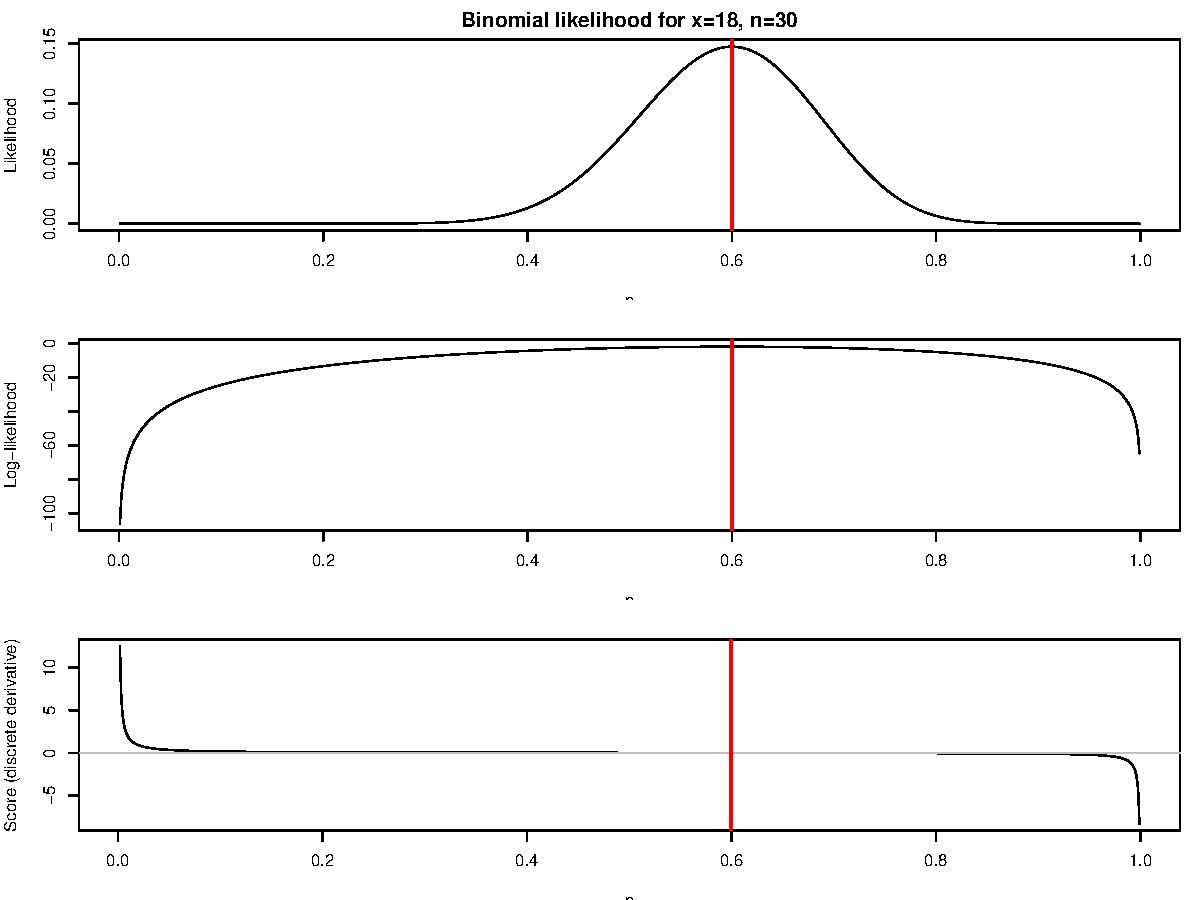
\includegraphics[keepaspectratio]{iter1_files/figure-beamer/fig-likelihood-1.pdf}}

}

\caption{\label{fig-likelihood}}

\end{figure}%
\end{frame}




\end{document}
